\documentclass{beamer}
%\usepackage{tikz}
\title{Implementing a clipboard interface under X11 - RCOS Presentation}
\date{July 21, 2015}
\author{Avi Weinstock}
\usepackage{fancyvrb}
\begin{document}
\maketitle

%\begin{frame}[fragile]
%\frametitle{An ideal interface}
%Ideally (for ease-of-use from an application programmer's perspective), an interface to the clipboard would looksomewhat like the following:
%\begin{Verbatim}[frame=single, fontsize=\scriptsize]
%status_code get_clipboard_contents(void* os_context,
%                                   char** output_data,
%                                   size_t* output_size);
%status_code set_clipboard_contents(void* os_context,
%                                   char* data,
%                                   size_t size);
%\end{Verbatim}
%\end{frame}
%
%\begin{frame}[fragile]
%\frametitle{X11 Cut Buffers}
%X11 does provide the following interface, which is close to the na\"ive/ideal interface:
%\begin{Verbatim}[frame=single, fontsize=\scriptsize]
%int XStoreBuffer(Display *display, char *bytes, int nbytes, int buffer);
%char *XFetchBuffer(Display *display, int *nbytes_return, int buffer);
%\end{Verbatim}
%\only<2>{However, cut buffers are deprecated...}
%\end{frame}

\begin{frame}[fragile]
\frametitle{Interface provided by rust-clipboard}
\begin{itemize}
\item
An intuitive mental model of clipboards is that there's a global, OS-managed blob of data, with \verb|get| and \verb|set| operations.
\item
This is not the case under X11 (and doesn't seem to be the case under Windows either, but seems like it might be the case under OSX).
\end{itemize}
\end{frame}

\begin{frame}[fragile]
\frametitle{Interface provided by rust-clipboard (continued)}
\begin{itemize}
\item
The goal of \verb|rust-clipboard| is to provide the simple/na\"ive get/set interface to the clipboard across all major OS's.
\item
\begin{Verbatim}[frame=single, fontsize=\scriptsize]
struct ClipboardContext; // innards are OS-dependent

impl ClipboardContext {
    pub fn new() -> Result<ClipboardContext, &str> { /* ... */ }
    pub fn get_contents(&self) ->
        Result<String, &str> { /* ... */ }
    pub fn set_contents(&self, data: String) ->
        Result<(), &str> { /* ... */ }
}
\end{Verbatim}
\end{itemize}
\end{frame}

\begin{frame}[fragile]
\frametitle{Example program using rust-clipboard}
\begin{Verbatim}[frame=single, fontsize=\scriptsize]
extern crate clipboard;
use clipboard::ClipboardContext;

fn main() {
    match ClipboardContext::new() {
        Ok(ctx) => {
            let data = ctx.get_contents().unwrap_or("");
            println!("Current clipboard contents: \"{}\"", data);
        },
        Err(msg) => {
            println!("Error initializing clipboard: {}", msg);
        }
    }
}
\end{Verbatim}
\end{frame}

\begin{frame}[fragile]
\frametitle{X Window System background}
\begin{columns}
\begin{column}{0.5\textwidth}
\begin{itemize}
\item
The X Window System was developed at MIT in 1984 as a successor to the W Window System.
\item
Clients communicate with the user (and each other) by sending events through the server.
\end{itemize}
\end{column}
\begin{column}{0.5\textwidth}
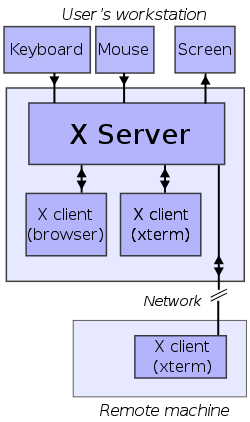
\includegraphics[height=0.8\textheight]{X_client_server_example.png}
\end{column}
\end{columns}
\footnotetext[1]{https://en.wikipedia.org/wiki/File:X\_client\_server\_example.svg}
\end{frame}

\begin{frame}[fragile]
\frametitle{X11 Clipboard protocol}
\begin{itemize}
\item
There is a simple mechanism for copying/pasting under X (called "cut buffers", accessed through \verb|XStoreBuffer| / \verb|XFetchBuffer|, but it's deprecated (due to performance reasons?).
\item
When a program "copies data to the clipboard" under X11, it actually starts a "server" process (an X client) that is responsible for \{streaming, chunking, format-negotiating\} the data with other X clients.
\item
"Retrieving data from the server" likewise involves sending messages to the current clipboard owner (the aforementioned "server").
\end{itemize}
\end{frame}

\begin{frame}[fragile]
\frametitle{The bug that took weeks to resolve}
\begin{itemize}
\item
My initial implementation of copy-to-clipboard seemed to cause paste actions to hang/timeout.
\item
According to print statements and \verb|ltrace|, all the values were the same in my program and \verb|xclip| (the C program I was using as a reference for the protocol) until the call to \verb|XNextEvent|, which "returned bogus data" (the event's "requestor" field showed up as my library, which then started responding to itself).
\end{itemize}
\end{frame}

\begin{frame}[fragile]
\frametitle{Sum types and tagged unions}
\begin{columns}
\begin{column}{0.5\textwidth}
\begin{itemize}
\item
Some languages have a feature called ADTs (Algebraic Data Types).
\item
Haskell:
\begin{Verbatim}[frame=single, fontsize=\scriptsize]
data Result t e = Ok t | Err e
\end{Verbatim}
\item
Rust:
\begin{Verbatim}[frame=single, fontsize=\scriptsize]
enum Result<T, E> {
    Ok(T), Err(E)
}
\end{Verbatim}
\end{itemize}
\end{column}
\begin{column}{0.5\textwidth}
\begin{itemize}
\item
In C, ADTs can be emulated with "tagged unions".
\item
\begin{Verbatim}[frame=single, fontsize=\scriptsize]
#define TAG_OK 0
#define TAG_ERR 1
struct result {
    int tag;
    union {
        void* ok;
        void* err;
    } value;
};
\end{Verbatim}
\item
Tagged unions don't (and can't) enforce that the field used is consistent with the tag.
\end{itemize}
\end{column}
\end{columns}
\end{frame}

\begin{frame}[fragile]
\frametitle{typedef union \_XEvent}
Xlib (the client library for X11) uses tagged unions for XEvent.
\begin{columns}
\begin{column}{0.5\textwidth}
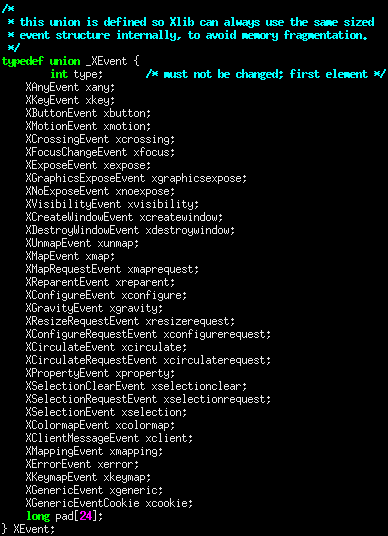
\includegraphics[height=0.8\textheight]{typedef_union_xevent.png}
\end{column}
\end{columns}
\end{frame}

\begin{frame}[fragile]
\frametitle{The bug that took weeks to resolve (resolved)}
\begin{itemize}
\item
It turns out that I was checking the tag on the XEvent, but then casting it to the wrong substructure.
\item
The fix was essentially this:
\begin{Verbatim}[frame=single, fontsize=\scriptsize]
  if evt.get_type() != SelectionRequest {
      return false;
  }
- let event: &XSelectionEvent        = unsafe { transmute(evt) };
+ let event: &XSelectionRequestEvent = unsafe { transmute(evt) };
\end{Verbatim}
\end{itemize}
\end{frame}

\begin{frame}[fragile]
\frametitle{Questions?}
\end{frame}

\begin{frame}[fragile]
\frametitle{Thanks}
\begin{itemize}
\item RCOS
\item Professor Goldschmidt
\item Professor Moorthy
\item The Mozilla Project
\item Sean O'Sullivan
\item Red Hat Incorporated
\end{itemize}
\end{frame}

\end{document}
